\documentclass[12pt,landscape]{article}
\usepackage{amsmath}
\usepackage{amsfonts}
\usepackage{bm}
\usepackage{color}
\usepackage{graphicx}
\definecolor{lyellow}{rgb}{0.97,0.94,0.8}
\definecolor{gray}{rgb}{0.4,0.4,0.4}

%\renewcommand{\baselinestretch}{1.2}

\textheight 18.5cm
\textwidth 24.5cm
\topmargin  -2.8cm
\oddsidemargin -0.8cm
\evensidemargin -0.8cm
%\pagestyle{empty}

%\partopsep -33pt
%\parsep 0pt
%\topskip -33pt
%\parskip 33pt


\newcommand{\lfrac}[2]{{\displaystyle\frac{{#1}}{{#2}}}}
\newcommand{\ffrac}[2]{{\textstyle\frac{{#1}}{{#2}}}}
\newcommand{\half}{\ffrac{1}{2}}



\newcommand{\I}{\mathrm{i}}
%\newcommand{\bld}[1]{\boldsymbol{#1}}
\newcommand{\cond}{\mbox{\rule[-0.5em]{.1mm}{1.2em}}}

%\renewcommand{\baselinestretch}{0.9}
\renewcommand{\topfraction}{0.8}
\renewcommand{\textfraction}{0.2}
\renewcommand{\floatpagefraction}{0.8}

\newcounter{denselistcounter}
\newenvironment{denselist}[1]
{ \begin{list}
  {#1{denselistcounter})}{\usecounter{denselistcounter}
  \setlength{\topsep}{-0pt}
  \setlength{\partopsep}{-0pt}
  \setlength{\itemsep}{-0pt}
  \setlength{\parsep}{-0pt}
  \setlength{\labelwidth}{6pt}
  \setlength{\labelsep}{4pt}
  \setlength{\leftmargin}{20pt}
  \setlength{\rightmargin}{20pt}
  }
}
{\end{list}}

\newcommand{\Bp}{\mathcal{B}_0}
\newcommand{\Bm}{\mathcal{B}_1}
\newcommand{\PGR}[1]{{\color{blue} #1}}

\begin{document}

\begin{center}
{\LARGE Unexpected large radii with finite folding}
\\[6pt]
{\large Discussion file: FAU -- MSU}
\\[3pt]
{\large Started: 2. August July 2025}
\\[3pt]
\end{center}

\centerline{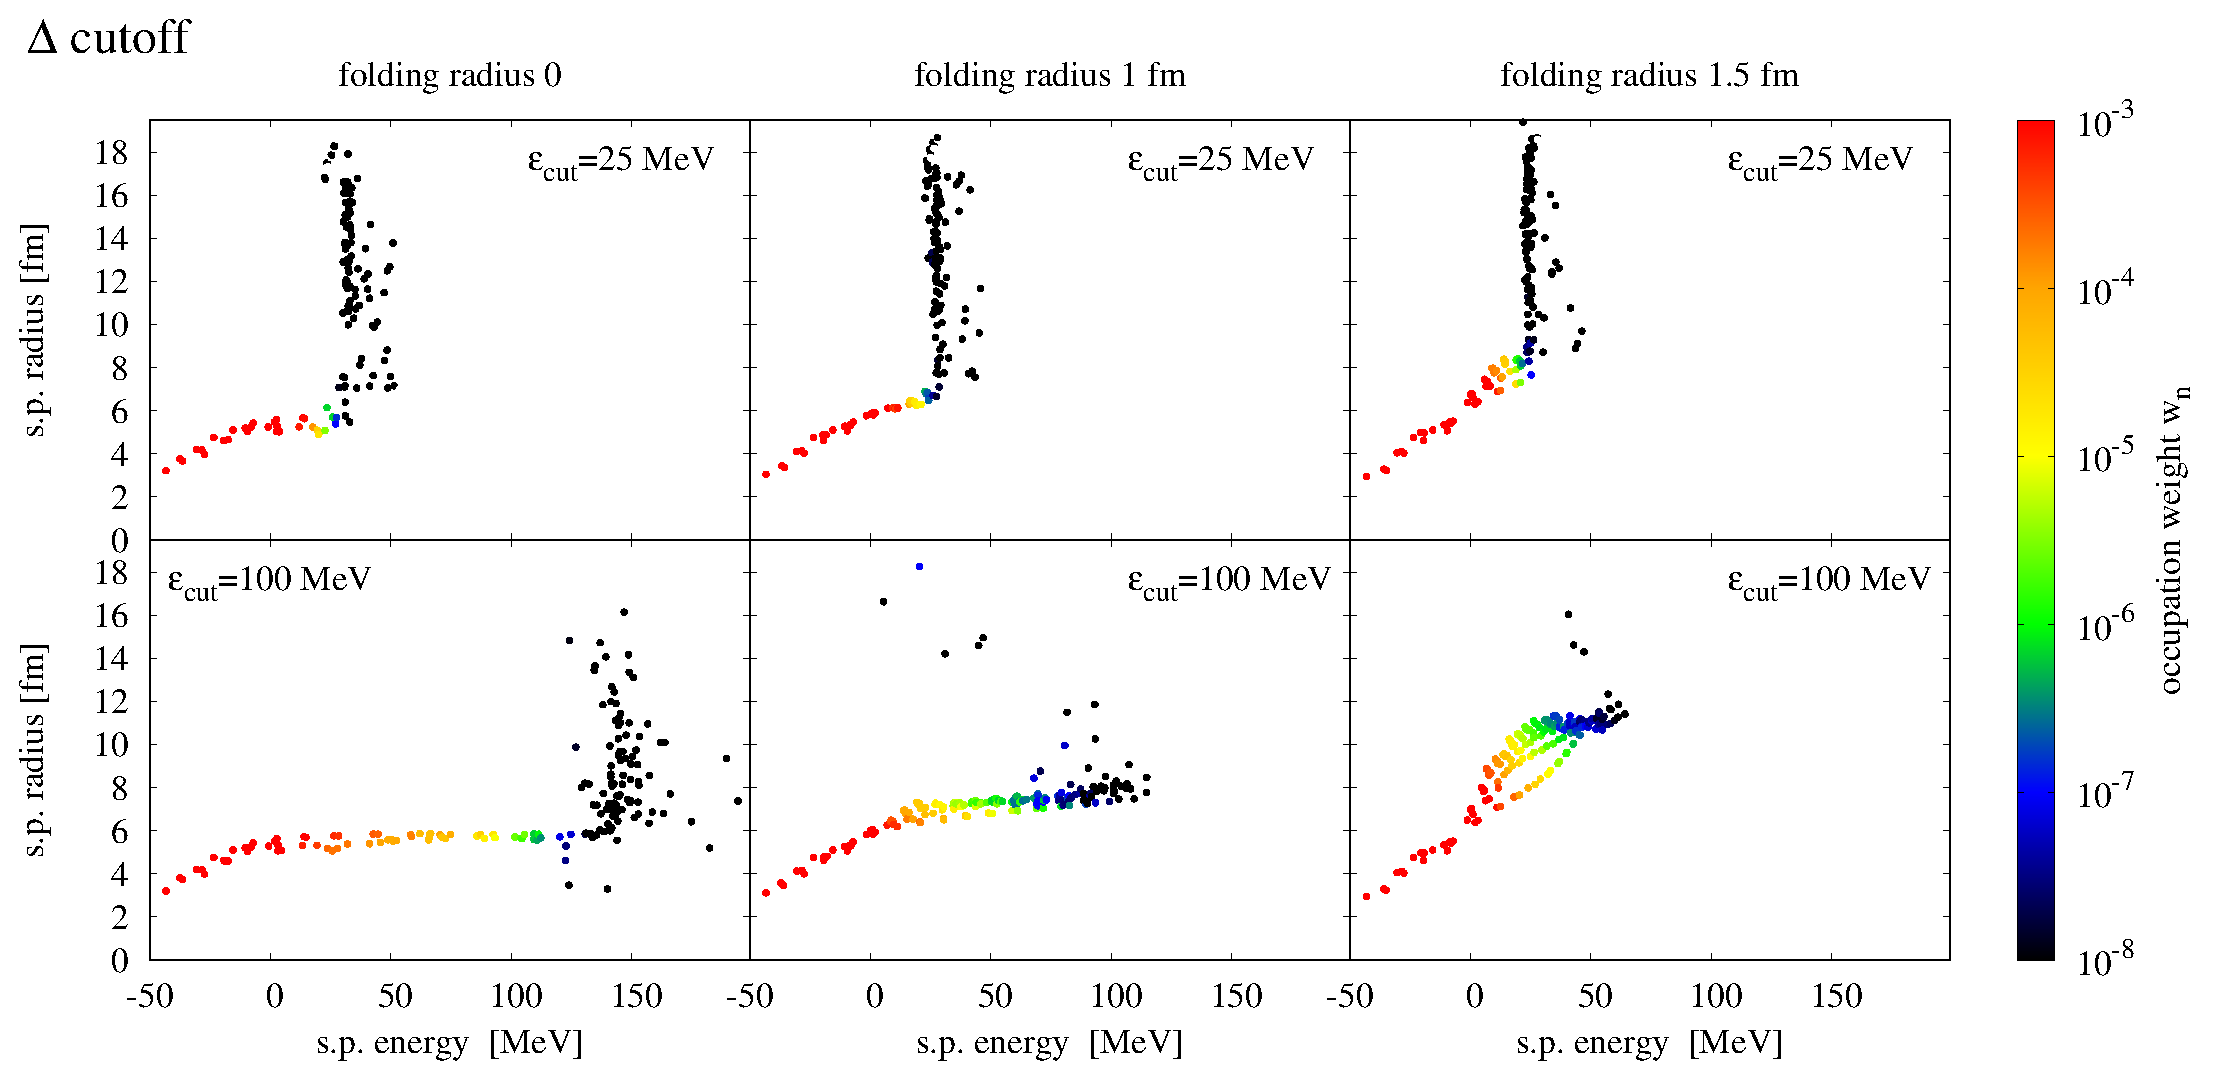
\includegraphics[width=0.99\linewidth]{testcut_uvspace}}

\medskip

The above figure shows the single-particle (s.p.) radii for neutrons
as function of the s.p. energy in $^{120}$Sn computed with SV-bas and
HFB pairing. The neutron pairing strength is tuned to produce a
pairing energy of about 12 MeV for each cutoff and folding radius. 
The actual occupation weights of the states are indicate by color
code.
\\
The figure shows that the unexpected (in connection with HFB) large
radii  come from inactive states (practically no occupation, indicated
by black). The comparison of two different cutoff energies shows that
the step increase of radii is connected to the cutoff energy which is
plausible. The figures look fine when omitting the inactive points.
\\
For the paper, we have decided for the 100 MeV cutoff to show a longer
s.p. energy scale. The older figure containing folding radius 1 fm was
done for a 25 MeV cutoff which was irritating as it amplifies the
inactive  states.

\newpage

\bigskip

\centerline{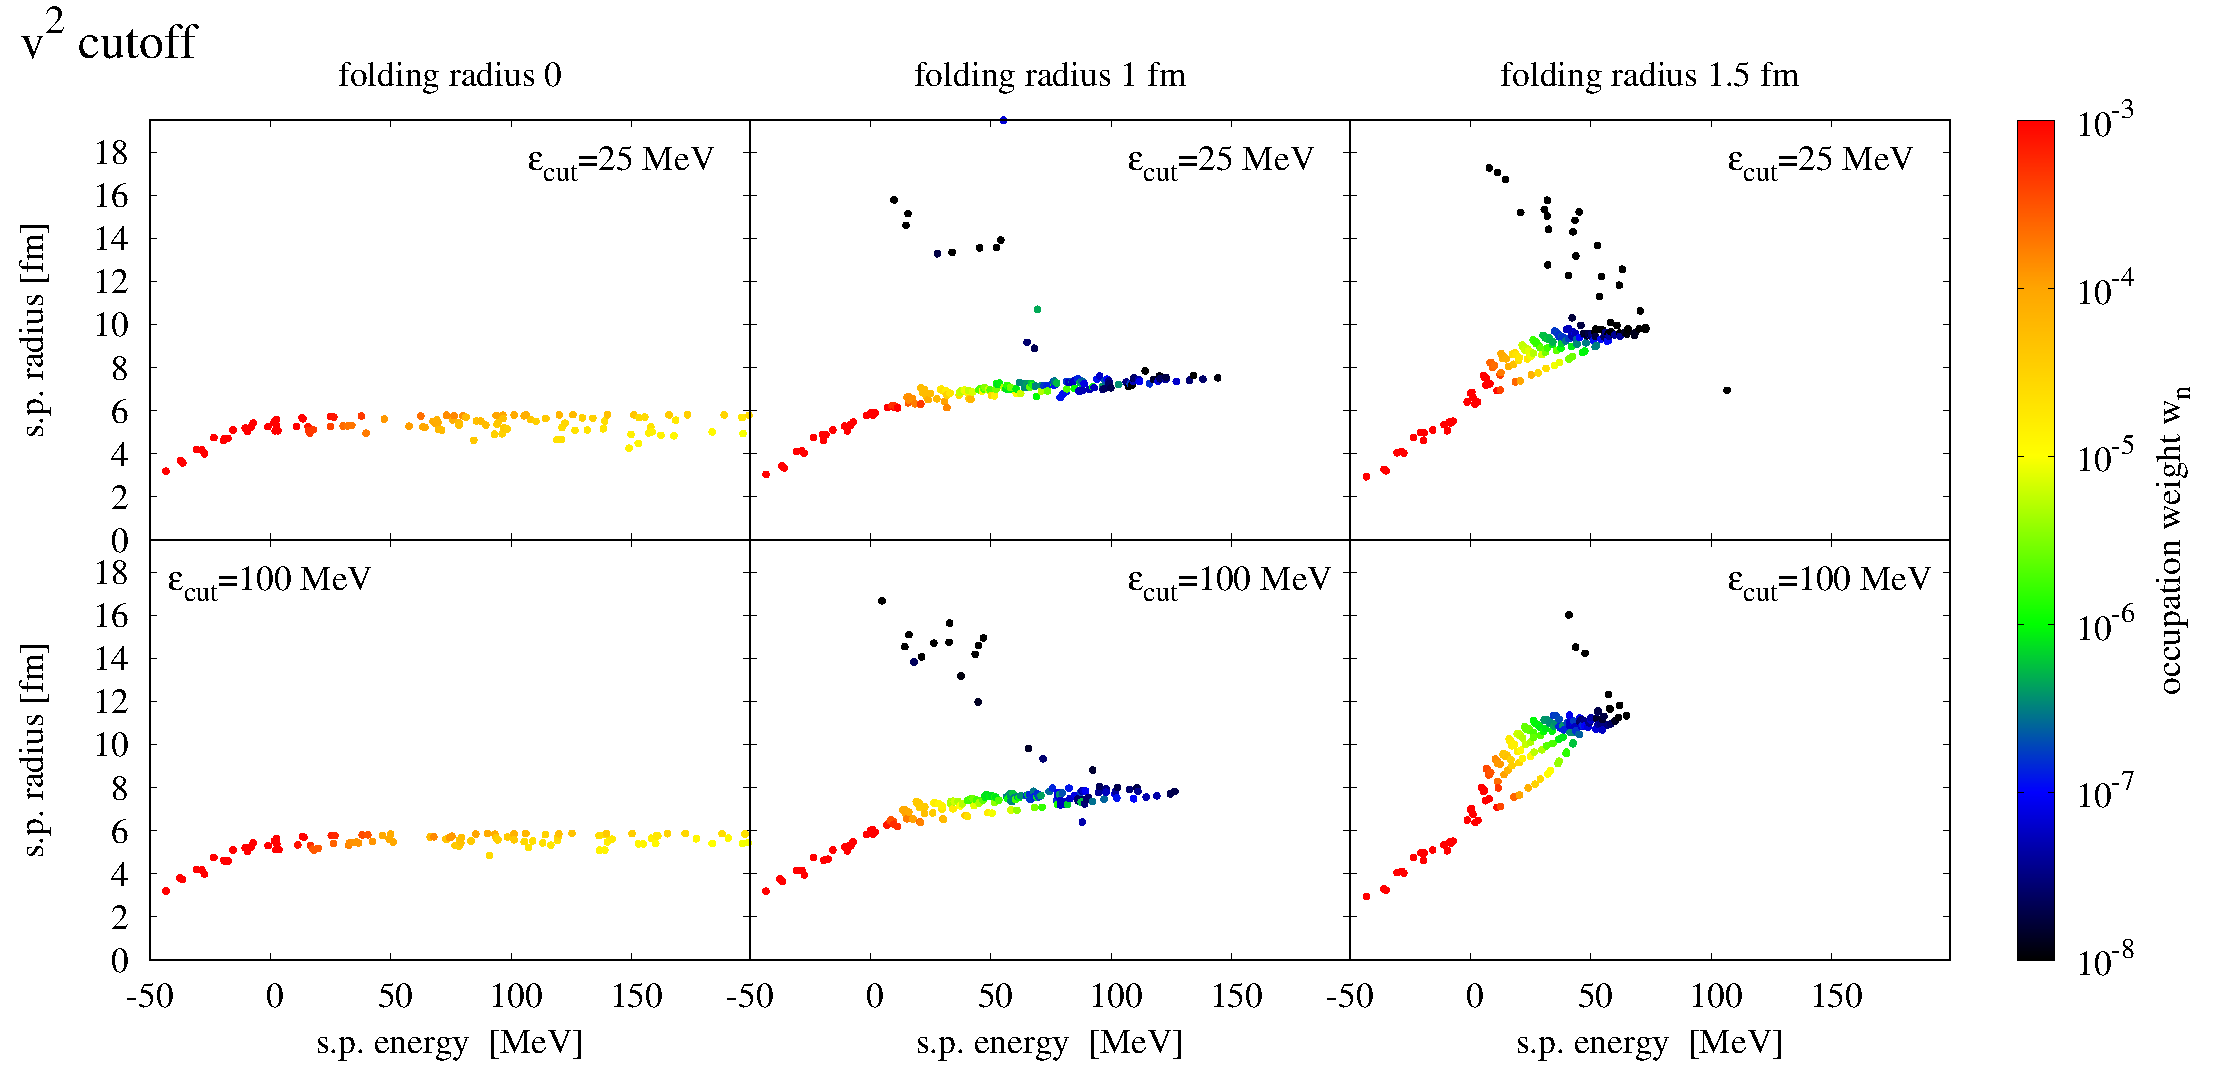
\includegraphics[width=0.99\linewidth]{testcut_v2space}}

\bigskip

There are two options for implementing the (soft) pairing cutoff.  The
first one, used on the previous page, goes through cutting the pairing
gap $\Delta$. The second option is to switch off all occupation
weights $v_n^2$. The above figure shows the trends of s.p. radii from
that option. It looks more gentle as it does not have the steep
increase of inactive state shortly above the cutoff energy. But it is
also not free of the problem. The inactive states are still spooking
around. For a good demonstration it is more important to use a large
cutoff energy and to hide the inactive states.

\end{document}
